\begin{frame}[containsverbatim]
	\frametitle{Motivating Example: Romano-British Pottery}

  Tubb, Parker \& Nicholson 
	analyzed the chemical composition of 26 samples of Romano-British
	pottery found at four kiln sites in Britain.
	\begin{itemize*}
		\item Sites: Ashley Rails, Caldicot, Isle of Thorns, Llanedryn
		\item Variables: aluminum (Al), iron (Fe), magnesium (Mg),
	calcium (Ca) and sodium (Na)
		\item $\rightarrow$ One-way MANOVA design, 4 groups, 5 responses
	\end{itemize*}
	
\begin{CodeInput}
R> library(heplots)
R> Pottery
\end{CodeInput}
\begin{CodeOutput}
          Site   Al   Fe   Mg   Ca   Na
1    Llanedyrn 14.4 7.00 4.30 0.15 0.51
2    Llanedyrn 13.8 7.08 3.43 0.12 0.17
3    Llanedyrn 14.6 7.09 3.88 0.13 0.20
 . . .
25 AshleyRails 14.8 2.74 0.67 0.03 0.05
26 AshleyRails 19.1 1.64 0.60 0.10 0.03
\end{CodeOutput} 

\end{frame}

\begin{frame}[containsverbatim]
	\frametitle{Motivating Example: Romano-British Pottery}
%\begin{uncoverenv}<1->
 \begin{block}{\textbf{Questions}:}
	\begin{itemize*}
	  \item \textbf{Can} the content of Al, Fe, Mg, Ca and Na  
	differentiate the sites?
	  \item \textbf{How to understand} the contributions of chemical elements
	  to discrimination?
	\end{itemize*}
\end{block}
%\end{uncoverenv}

%\begin{uncoverenv}<2->
\black{\textbf{Numerical answers}}:
\begin{CodeInput}
R> pottery.mod <- lm(cbind(Al, Fe, Mg, Ca, Na) ~ Site)
R> Manova(pottery.mod)
\end{CodeInput}
\begin{CodeOutput}
Type II MANOVA Tests: Pillai test statistic
     Df test stat approx F num Df den Df  Pr(>F)    
Site  3      1.55     4.30     15     60 2.4e-05 ***
---
Signif. codes:  0 '***' 0.001 '**' 0.01 '*' 0.05 '.' 0.1 ' ' 1 
\end{CodeOutput} 
%\end{uncoverenv}

%\begin{uncoverenv}<3->
\black{\textbf{What have we learned?}}
	\begin{itemize*}
		\item \textbf{Can}: YES! We can discriminate sites.
		\item But: \textbf{How to understand} the pattern(s) of group differences: ???
	\end{itemize*}
%\end{uncoverenv}
\end{frame}

\begin{frame}
	\frametitle{Motivating Example: Romano-British Pottery}
%	\framesubtitle{Visual answer: HE plots}
  \begin{block}{Univariate plots are limited}
  	\begin{itemize*}
  	\item Do not show the \emph{relations} of variables to each other
    \end{itemize*}
  \end{block}
 	\begin{center}
 	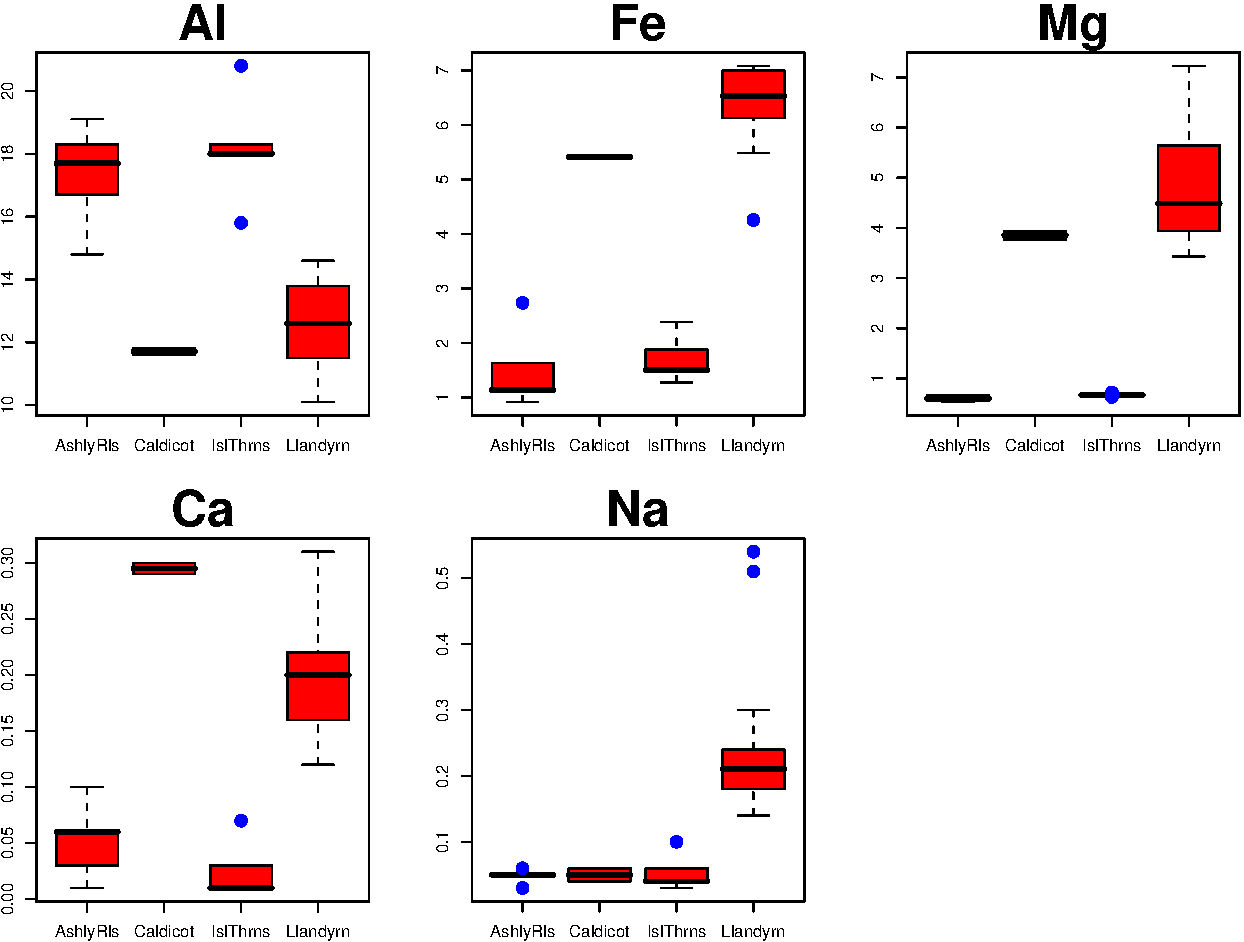
\includegraphics[width=.6\textwidth,clip]{fig/pottery-box}
 	\end{center}
	
\end{frame}

\begin{frame}[containsverbatim]
	\frametitle{Motivating Example: Romano-British Pottery}
%	\framesubtitle{Visual answer: HE plots}
\begin{columns}[c]
 \begin{column}{0.5\textwidth}
  \begin{block}{Visual answer: HE plot}
%  \textbf{Visual answer}: HE plot
  \begin{itemize}
  	\item Shows variation of means (\mat{H}) relative to residual
  	(\mat{E}) variation
  	\item Size and orientation of \mat{H} wrt \mat{E}: \emph{how much}
  	and \emph{how} variables contribute to discrimination
  	\item Evidence scaling: \mat{H} is scaled so that it projects
  	outside \mat{E} \emph{iff} null hypothesis is rejected.
	\end{itemize}
 \end{block}
%	\href{file://heplot-movie.ppt}{\beamerbutton{heplot-movie.ppt}}
%	\href{file://pottery0.gif}{\beamerbutton{pottery0.gif}}
  \href{run:powerpoint.bat}{\beamerbutton{Run heplot-movie.ppt}}
 \end{column}
 \begin{column}{0.5\textwidth}
 	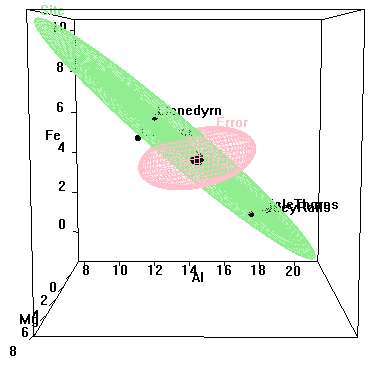
\includegraphics[width=\textwidth,clip]{fig/pottery0-3d}
  \begin{CodeInput}
  R> heplot3d(pottery.mod)
  \end{CodeInput}
 \end{column}
\end{columns}
	
\end{frame}

\begin{frame}<none>[containsverbatim]
	\frametitle{Motivating Example: Romano-British Pottery}
%	\framesubtitle{Visual answer: HE plots}
\begin{columns}
 \begin{column}{0.5\textwidth}
  \begin{block}{Visual answer: HE plot}
%  \textbf{Visual answer}: HE plot
  \begin{itemize}
  	\item Shows variation of means (\mat{H}) relative to residual
  	(\mat{E}) variation
  	\item Size and orientation of \mat{H} wrt \mat{E}: \emph{how much}
  	and \emph{how} variables contribute to discrimination
  	\item Evidence scaling: \mat{H} is scaled so that it projects
  	outside \mat{E} \emph{iff} null hypothesis is rejected.
	\end{itemize}
 \end{block}
%	\href{file://heplot-movie.ppt}{\beamerbutton{heplot-movie.ppt}}
%	\href{file://pottery0.gif}{\beamerbutton{pottery0.gif}}
  \href{run:powerpoint.bat}{\beamerbutton{Run heplot-movie.ppt}}
 \end{column}
 \begin{column}{0.5\textwidth}
 	\movie[width=\textwidth,height=\textwidth,poster,showcontrols,loop]{}{pottery0.mpg}
  \begin{CodeInput}
  R> heplot3d(pottery.mod)
  \end{CodeInput}
 \end{column}
\end{columns}
	
\end{frame}


